% !TEX root = pfe-book1.tex
%!TEX TS-program = pdflatex
%!TEX encoding = UTF-8 Unicode


\cleardoublepage
\chapter{Oscillations}


\section{Equilibrium}


In certain cases it is very difficult to maintain an equilibrium -- try to walk across a tightrope. At the same time,
nobody rewards a person sitting in a rocking-chair with
applause. But he is also maintaining his equilibrium.

What is the difference between these two examples?
In which case is equilibrium maintained ``by itself''?

The condition for equilibrium seems to be obvious. For
a body not to be displaced from its position, the forces
exerted on it must balance; in other words, the sum of
these forces must be equal to zero. This condition is
really necessary for the equilibrium of a body, but is it
sufficient?

A side-view of a hill easily built out of cardboard paper
is depicted in \figr{fig-4.01}. A ball will behave in different
ways depending on the part of the hill where it is placed. A force which makes it roll down will be exerted on the
ball at any point on the slope of the hill. This active force
is gravity, or rather its projection on the tangent to the
section of the hill passing through the point which is of
interest to us. It is therefore clear that the more gentle
the slope, the smaller the force acting on the ball.

\begin{figure}[!ht]
\centering

\includegraphics[width=0.6\textwidth]{figures/fig-04-01.pdf}
\caption{A ball on a cardboard hill.}
\label{fig-4.01}
\end{figure}

We are interested above all in the points at which the
force of gravity is completely balanced by the reaction
of the support, and hence the resultant force acting on
the ball is equal to zero. This condition will be fulfilled
at the top of the hill and at its lowest points-the hollows.

The tangents are horizontal at these points, and the resultant forces acting on the ball are equal to zero.

However, in spite of the fact that the resultant force
is equal to zero at the top, we won't be able to put a ball
there, but even if we could, we would immediately detect
the accessory cause of our success -- friction. A small
push or a light puff will overcome the frictional force, and
the ball will leave its place and roll down.

For a smooth ball on a smooth hill, only the low points
of the hollows will be positions of equilibrium. If a
push or an air stream displaces the ball from such a position, it will return there by itself.

A body in a hollow (a hole or a depression) is undoubtedly in equilibrium. If we deflect it from such a position,
a force returns it back. The picture is different at the top
of the hill: if a body has left such a position, the force
exerted on it tends to take it further away rather than
bring it back. Consequently, the resultant force equal to
zero, is a necessary but not a sufficient condition for stable
equilibrium.

The equilibrium of a ball on a hill can also be regarded
from another point of view. The hollows correspond to
minima, and the top to maxima of potential energy. The
law of conservation of energy prevents a change in positions for which the potential energy is minimum. Such a change would make the kinetic energy negative, which however, is impossible. The situation is entirely different at the top. A departure from these points entails a decrease in potential energy, and hence not a decrease, but
an increase in kinetic energy.

Thus, in a position of equilibrium, the potential energy
must assume a minimum value with respect to its values
at neighbouring points.

The deeper the hole, the greater will be the stability.
Since we know the law of conservation of energy, we can
immediately say under what conditions a body will roll
out of a depression. For this it is necessary to impart to
the body the kinetic energy which would be enough for
raising it to the edge of the hole. The deeper the hole,
the greater will be the kinetic energy needed for disturbing
the stable equilibrium.

\section{Simple Oscillations}

If a ball lying in a depression is pushed, it will begin
moving up the hill, gradually losing its kinetic energy.
When it is completely lost, an instantaneous halt will
occur and a downward motion will begin. Its potential
energy will now be transformed into kinetic one. The
ball will gain speed, rush past the equilibrium position
by inertia and begin ascending again, only in the opposite
direction. If the friction is insignificant, such an ``upward-downward'' motion can continue very long, while
in the ideal case-in the absence of friction -- it will continue indefinitely.

Therefore, motions near the position of stable equilibrium always have an oscillatory nature.

For studying oscillation, a pendulum is perhaps more
suitable than a ball rolling back and forth in a hole, at
least to the extent that it is easier to reduce the friction
exerted on a pendulum to a minimum.

When a pendulum bob is deflected to its highest position, its speed and kinetic energy are equal to zero. Its
potential energy is greatest at this moment. The bob goes
down -- the potential energy decreases and is transformed
into kinetic one. Hence, the speed of the motion increases
too. When the bob passes through its lowest position, its
potential energy is least, and correspondingly the kinetic energy and speed are maximum. As the motion continues, the bob again rises. The speed now diminishes and the potential energy increases.

If we abstract from the friction losses, the bob will
be deflected by the same distance to the right as it was
originally deflected to the left. Its potential energy was
transformed into kinetic one and then the same amount of
``new'' potential energy was created. We have described the
first half of a single oscillation. The second half takes
place in the same way, only the bob moves in the opposite
direction.

Oscillatory motion is a repeating or, as one says, periodic motion. Returning to its starting point, the bob repeats its motion each time (if the changes resulting from friction are not taken into account) both with respect to its path and to its velocity and acceleration. The time spent on a single oscillation, i.e. in returning to the starting point, is identical for the first, second and all subsequent oscillations. This time -- one of the most important characteristics of an oscillation is called the \emph{period}; we shall denote it by $T$. After this time, the motion is repeated, i.e, after the time $T$, we shall always find a vibrating body at the same point in space and moving in the same direction. After a half-period, the displacement of the body and also the direction of the motion change sign. Since the period $T$ is the time for one oscillation, the number $n$ of oscillations in a unit of time will be equal to $1/T$.


\begin{figure}[!ht]
\centering
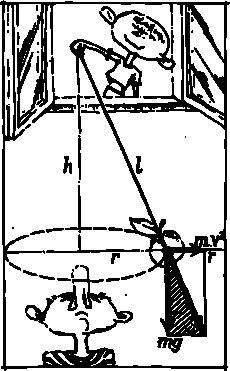
\includegraphics[width=0.5\textwidth]{figures/fig-04-02.pdf}
\caption{Analysing the motion of a ``conical pendulum''.}
\label{fig-4.02}
\end{figure}

But what does the period of vibration of a body moving
not far from the position of stable equilibrium depend on?
In particular, what does the period of oscillation of a
pendulum depend on? Galileo was the first to pose and
solve this problem. We shall now derive Galileo's formula.

However, it is difficult to apply the laws of mechanics
to non-uniformly accelerated motion in an elementary
manner. Therefore, in order to bypass this difficulty, we
shall not make the pendulum bob oscillate in a vertical
plane, but have it describe a circle, remaining at a fixed
height all the time. It isn't difficult to create such a
motion-one merely has to remove the pendulum from its
equilibrium position and give it an initial push with
a properly chosen force in the direction exactly perpendicular to the radius of deflection.

Such a ``conical pendulum'' is depicted in \figr{fig-4.02}.

The bob of mass $m$ moves around a circle. Hence, besides
the force of gravity $mg$, a centrifugal force of $mv^{2}/r$,
which we may also represent in the form $4 \pi^{2} n^{2} rm$
is exerted on it. Here $n$ is the number of revolutions per
second. We may therefore also write out our expression
for the centrifugal force as follows: $4 \pi^{2} rm/T^{2}$. The resultant of these two forces pulls on the cord of the pendulum.

Two similar triangles -- the force triangle and the
distance triangle -- are shaded in the figure. The ratios of
the corresponding legs are equal; hence
\begin{equation*}%
\frac{mgT^{2}}{4 \pi^{2}rm} = \frac{h}{r}\,\, \textrm{or} \,\,
T = 2 \pi \sqrt{\frac{h}{g}}
\end{equation*}
What factors does the period of oscillation of a pendulum depend on? If we perform experiments at one and the same location on the Earth ($g$ doesn't change), the period of oscillation depends only on the difference in height between the point of suspension and the point
where the bob is. The mass of the bob, as always in a gravitational field, does not affect the period of oscillation.

The following circumstance is of interest. We are
investigating motion near the position of stable equilibrium. For small deflections, we may replace the difference in height $h$ by the length $l$ of the pendulum. It is easy to verify this. If the length of the pendulum is \SI{1}{\meter} and the radius of deflection is \SI{1}{\centi\meter}, then 
\begin{equation*}%
h = \sqrt{\num{10 000} - 1} = \SI{99.995}{\centi\meter}
\end{equation*}
The difference between $h$ and $l$ will reach 1\% only when
the deflection is \SI{14}{\centi\meter}. Consequently, the period of the
free oscillations of a pendulum for not too large a deflection from the equilibrium position is
\begin{equation*}%
T = 2 \pi \sqrt{\frac{l}{g}}
\end{equation*}
i.e. depends only on the length of the pendulum and the
value of the acceleration of free fall at the place where the
experiment is performed, but does not depend on the
magnitude of the deflection of the pendulum from equilibrium position.

The formula $T = 2\pi \sqrt{l/g}$ has been proved for a conical
pendulum. What will it look like for a simple ``plane''
pendulum? It turns out that this formula retains its
form. We shall not prove this rigorously, but call attention to the fact that the shadow cast onto a wall by the bob of a conical pendulum will oscillate almost like a plane pendulum: the shadow completes one oscillation during just the same time in which the bob describes
a circle.

The use of small oscillations about an equilibrium
position permits the measurement of time with very
great accuracy.

According to legend, Galileo established the independence of the period of oscillation of a pendulum of its amplitude and mass while observing during services in a cathedral how two enormous chandeliers were swinging.

Therefore, the period of oscillation of a pendulum is proportional to the square root of its length. Thus, the period of oscillation of a metre-long pendulum is twice that of a \SI{25}{\centi\meter} pendulum. It also follows from our formula for the period of oscillation of a pendulum that one and the same pendulum will not oscillate equally fast
at different latitudes on the Earth. As we move closer to the equator, the acceleration of free fall decreases and the period of oscillation grows.

It is possible to measure a period of oscillation with a
very great degree of accuracy. Therefore, experiments
with pendulums enable us to measure the acceleration
of free fall very accurately.

\section{Displaying Oscillations}
Let us attach a piece of soft lead to the bob of a pendulum and hang the pendulum over a sheet of paper in such a way that the lead touches the paper (\figr{fig-4.03}).

\begin{figure}[!ht]
\centering
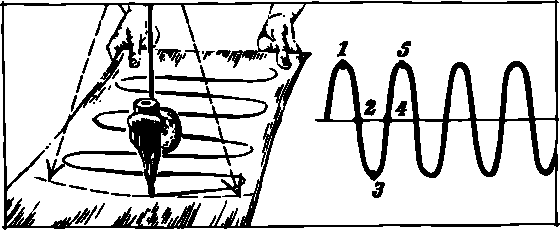
\includegraphics[width=\textwidth]{figures/fig-04-03.pdf}
\caption{Tracing the trajectory of the pendulum.}
\label{fig-4.03}
\end{figure}

Now we deflect the pendulum slightly. The oscillating
lead will trace a small line segment on the paper. At the
midpoint of the oscillation, when the pendulum is passing through its equilibrium position, the pencil line will
be thicker, since in this position the lead presses down
harder on the paper. If we pull the sheet of paper in the
direction perpendicular to the plane of the oscillation,
the curve depicted in \figr{fig-4.03} will be traced. It is not
difficult to see that the wavelets so obtained will be
dense if the paper is pulled slowly, and sparse if the
sheet of paper moves with a considerable speed. In order
for the curve to turn out accurate, it is necessary that
the sheet of paper move uniformly.

In this manner we have in a sense ``displayed'' the
oscillations.

The display is needed in order to say where the bob of
the pendulum was located and where it was moving at
one or another instant. Imagine that the paper moves
with a speed of \SI{1}{\centi\meter\per\second} from the time when the pendulum was as far as possible from, say, to the left of, the midpoint. This initial position corresponds to the point on our graph which has been marked with the number \textbf{1}.

After a quarter of the period the pendulum will pass
through the midpoint. During this time the paper has
moved $T/4$ centimetres (point \textbf{2} in the figure). The pendulum now moves to the right and the paper simultaneously crawls along. When the pendulum comes to its extreme right position, the paper will have moved $T/2$ centimetres (point \textbf{3} in the figure). The pendulum again moves towards the midpoint and arrives at its equilibrium position in $3T/4$ (point \textbf{4} in the diagram). Point \textbf{5} finishes a complete oscillation, after which the motion is repeated every $T$ seconds or every $T$ centimetres on our graph.

Thus, a vertical line on the graph is the scale of the
displacement of a point from the equilibrium position,
and the central horizontal line is the time scale.

The two quantities which characterize an oscillation
in an exhaustive manner are easily found from such
a graph. The period can be determined by the distance
between two equivalent points, for example, between
two neighbouring summits. The maximum displacement
of a point from the equilibrium position can also be
measured at once. This displacement is called the \emph{amplitude} of the oscillation.

Displaying an oscillation permits us, moreover, to
answer the question posed above: Where is an oscillating
point at one or another instant? For example, where will
an oscillating point be in 11 seconds if the period of
oscillation is equal to 3 seconds and the motion began
at the extreme left position? The oscillation begins from
the very same point in every 3 seconds. Therefore, in
9 seconds the body will also be at the extreme left position.

Consequently, there is no need of a graph in which the
curve is extended over several periods; a graph depicting
the curve corresponding to one oscillation is quite enough.
In 11 seconds the state of an oscillating point will be
the same as in 2 seconds if the period is 3 seconds. Laying
off 2 centimetres in our diagram (for we stipulated that
the paper be pulled with a speed of  \SI{1}{\centi\meter\per\second} or, in other words, that the scale of our diagram be 1 second to 1 centimetre), we see that in 11 seconds the point will be on 	its way from the extreme right position to that of equilibrium. The magnitude of the displacement at this instant can be found from the figure.

It isn't necessary to turn to a graph in order to find
the magnitude of the displacement of a point making
small oscillations about its equilibrium position. Theory
shows that in this case the curve depicting the dependence
of the displacement on the time is a sinusoid. If we denote
the displacement of a point by $y$, the amplitude by $a$,
and the period of the oscillation by $T$, we can find the
magnitude of the displacement at a time $t$ after the beginning of the oscillation by means of the formula:
\begin{equation*}%
A = a \sin 2 \pi \frac{t}{T}
\end{equation*}
An oscillation taking place in accordance with this law
is called \emph{harmonic}. The argument of the sine is equal to
the product of $2\pi$ by $t/T$. The quantity $2 \pi t/T$ is called
the \emph{phase}.

Having trigonometric tables at hand and knowing the
period and amplitude, we can easily compute the magnitude of the displacement of a point, and figure out on the basis of the value of the phase in which direction it is moving.

It is not difficult to derive the formula for vibratory
motion by considering the motion of the shadow cast on a
wall by a bob moving around a circle (\figr{fig-4.04}).

\begin{figure}[!ht]
\centering
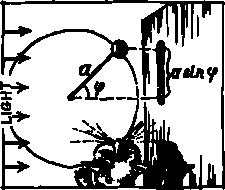
\includegraphics[width=0.6\textwidth]{figures/fig-04-04.pdf}
\caption{Analysing the motion of a shadow cast on a wall by a bob moving around a circle.}
\label{fig-4.04}
\end{figure}

We shall mark off the displacements of the shadow from
its central position. At the extreme positions the displacement $y$ is equal to the radius $a$ of the circle. This is the amplitude of the oscillation of the shadow.

If the bob has moved along the circle through an angle $\varphi$ from the central position, its shadow will deviate from
the midpoint by $a \sin (\varphi)$.

Let the period of the motion of the bob (which, of
course, is also the period of oscillation of the shadow)
be $T$; this means that the bob passes through $2\pi$ radians
during the time $T$. We may form the proportion $\varphi/t = 2\pi/T$, where $t$ is the time required for a revolution
through an angle $\varphi$.

Consequently, $\varphi = 2\pi t /T$ and $y = a \sin 2 \pi t/T$. This is
precisely what we wished to prove.

The velocity of an oscillating point also changes
according to a sinusoidal law. The same kind of reasoning about the movement of the shadow of a bob describing
a circle will lead us to this conclusion. The velocity of
the bob is a vector of constant length $v_{0}$. The velocity
vector revolves together with the bob. Let us think of
the velocity vector as a physical arrow capable of casting
a shadow. At the extreme positions of the bob, the vector
will lie along a ray of light and will not create a shadow.

When the bob moves around the circle from an extreme
position through an angle $\theta$, the vector velocity will
turn through the same angle and its projection will be
equal to $v_{0} \sin \theta$. But on the same basis as before, $\theta /t = 2\pi/T$ and so the instantaneous speed of the vibrating body
\begin{equation*}%
v = v_{0} \sin \frac{2\pi}{T} t
\end{equation*}
Note that in the formula for determining the magnitude
of the displacement, the time is equal to zero at the
central position, and in the formula for the speed at the
extreme positions. The displacement of a pendulum equals
zero when the bob is at the central position, and the
speed of oscillation is zero at the extreme positions.

There is a simple relation between the maximum speed $v_{0}$ of an oscillation and the maximum displacement (or amplitude): the bob describes a circle with a circumference $2 \pi a$ during the period $T$ of the oscillation. Therefore,
\begin{equation*}%
v_{0} = \frac{2\pi a}{T} \,\,\textrm{and}\,\,v=\frac{2 \pi a}{T} \sin \frac{2 \pi}{T} t
\end{equation*}

\section{Force and Potential Energy in Oscillations}

During every oscillation about an equilibrium position,
there is a force acting on the vibrating body ``desiring''
to return it to the equilibrium position. When a point
is receding from its equilibrium position, the force
decelerates its motion; when it is approaching this position, the force accelerates its motion.

Let us examine this force in the case of a pendulum
(\figr{fig-4.05}). The bob of the pendulum is acted upon by
the force of gravity and tension in the string. Let us
decompose the force of gravity into two components --
one directed along the string and the other perpendicular
to it, along the tangent to the path. Only the tangential
component of the gravitational force is of significance for
the motion. I t is precisely the restoring force in this case.
As for the force directed along the string, it is balanced
by the reaction on the part of the nail on which the pendulum is hanging, and it is only necessary to take it
into account when we are interested in whether the string
will withstand the weight of the vibrating body.
\begin{figure}[!ht]
\centering
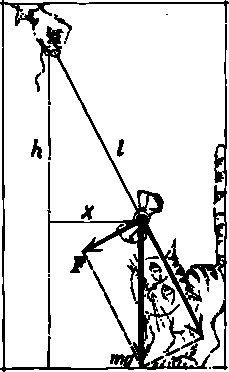
\includegraphics[width=0.6\textwidth]{figures/fig-04-05.pdf}
\caption{Analysing restoring force for a pendulum.}
\label{fig-4.05}
\end{figure}

Denote the magnitude of the displacement of the bob
by $x$. The motion takes place along an arc, but we have
agreed to investigate oscillations near an equilibrium
position. We therefore make no distinction between the
magnitude of a displacement along the arc and the deviation of the bob from the vertical. Let us consider two similar triangles. The ratio of the corresponding legs is equal to the ratio of the hypotenuses, i.e.
\begin{equation*}%
\frac{F}{x} = \frac{mg}{l}, \,\,\textrm{or}\,\,F = \frac{mg}{l}x
\end{equation*}
The quantity $mg/l$ does not change during the oscillation. If we denote this constant by $k$, then the restoring force $F$ is given by the formula $F = kx$. We arrive at the following conclusion: the magnitude of the restoring force is directly proportional to that of the displacement of an oscillating point from its equilibrium position. The restoring force is maximum at the extreme positions
of a vibrating body. When the body passes through the
midpoint, the force vanishes and changes sign or, in
other words, direction. While the body is displaced to
the right, the force is directed to the left, and conversely.

The pendulum serves as the simplest example of an
oscillating body. However, we are interested in the possibility of extending the formulas and laws which we
find to arbitrary vibrations.

The period of oscillation of a pendulum was expressed
in terms of its length. Such a formula applies only to
a pendulum. But we can express the period of free oscillations in terms of the restoring force constant $k$. Since $k = mg/l$, we have
$l/g= m/k$, and so 
\begin{equation*}%
T = 2 \pi \sqrt{\frac{m}{k}}
\end{equation*}
\label{pend-osc}
This formula extends to all cases of oscillations, since
any free oscillation takes place under the action of a restoring force.

Let us now express the potential energy of a pendulum
in terms of its displacement $x$ from the equilibrium position. We may take the potential energy of the bob to be zero when it passes through the lowest point, and then the height of its ascent should be measured from this point. Denoting the difference in height between the point of suspension and the level of the deflected bob by $h$, we express the potential energy as follows: $U = mg (l - h)$ or, using the formula for the difference of squares,
\begin{equation*}%
U = mg \frac{l^{2}-h^{2}}{l+h}
\end{equation*}
But, as can be seen from the figure, $l^{2} -h^{2} = x^{2}$, $l$ and
$h$ differ very slightly and, therefore, $2l$ may be substituted for $l
+ h$. Thus, $U = mgx^{2}/2l$
\begin{equation*}%
U = \frac{kx^{2}}{2}
\end{equation*}
The potential energy of an oscillating body is proportional to the square of its displacement from the equilibrium position.

Let us check the correctness of the formula we have just
derived. The loss of potential energy must be equal to the
work performed by the restoring force. Consider two of the
body's positions, $x_{2}$ and $x_{1}$. The difference in potential
energy
\begin{equation*}%
U_{2} - U_{1} = \frac{k x_{2}^{2}}{2} -  \frac{k x_{1}^{2}}{2} = \frac{k}{2} \left(x_{2}^{2} - x_{1}^{2} \right)
\end{equation*}
But a difference of squares may be written as the product of the sum by the difference. Hence,
\begin{equation*}%
U_{2} - U_{1} = \frac{k}{2} (x_{2} + x_{1})(x_{2} - x_{1}) = \frac{kx_{2}+kx_{1}}{2} (x_{2}-x_{1})
\end{equation*}
$x_{2}-x_{1}$ is the length of the path covered by the body,
and $kx_{1}$ and $kx_{2}$ are the magnitudes of the restoring force at
the beginning and end of the motion, and $(kx_{1}+kx_{2})/2$
is equal to the average force.

Our formula led us to the correct result: the loss of
potential energy is equal to the work performed.

\section{Spring Vibrations}
It is easy to make a ball oscillate by hanging it on a
spring. Let us fasten one end of the spring and pull the
ball (\figr{fig-4.06}). The spring will be in a stretched position as long as we pull the ball with our hand. If we
let go, the spring will unstretch and the ball will begin
moving towards its equilibrium position. Just as the
pendulum, the spring will not come to a state of rest
immediately. The equilibrium position will be passed by
inertia, and the spring will begin compressing. The ball
slows down, and at a certain instant it comes to a halt in
order to start moving at once in the opposite direction.
There arises an oscillation with the same typical features
with which our study of the pendulum acquainted us.

In the absence of friction, the oscillation would continue indefinitely. In the presence of friction, the oscillations are damped; moreover, the greater the friction, the faster they are damped.

\begin{figure}[!ht]
\centering
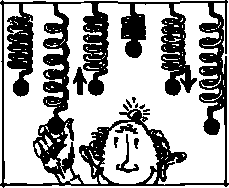
\includegraphics[width=0.6\textwidth]{figures/fig-04-06.pdf}
\caption{The action and reaction.}
\label{fig-4.06}
\end{figure}

The roles of a spring and a pendulum are frequently
analogous. Both one and the other serve to maintain constancy in the period of clocks. The precise movement of
modern spring watches is ensured by the oscillatory motion of a small flywheel balance. It is set oscillating by a
spring which winds and unwinds tens of thousands of
times a day.

For the ball on a string, the role of the restoring force
was played by the tangential component of gravity. For
the ball on a spring, the restoring force is the elastic force
of a contracted or stretched spring. Therefore, the magnitude of the elastic force is directly proportional to the
displacement: $F = kx$.

The coefficient $k$ has another meaning in this case. It
is now the stiffness of the spring. A stiff spring is one which
is difficult to stretch or contract. The coefficient $k$ has
precisely such a meaning. The following is clear from the
formula: $k$ is equal to the force necessary for the stretching or contraction of the spring by a unit of length.

Knowing the stiffness of the spring and the mass of
the load hung on it, we find the period of free oscillation
with the aid of the formula $T = 2 \pi \sqrt{m/k}$. For example,
a load of mass \SI{10}{\gram} on a spring with a stiffness coefficient \num{d5} dyn/cm (this is a rather stiff spring-a hundred-gram weight will stretch it by \SI{1}{\centi\meter}) will oscillate with a period $T = \SI{6.28d-2}{\second}$. During one second, 16 oscillations will take place.

The more flexible the spring, the slower will be the
vibration. An increase in the mass of the load has the
same effect.

Let us apply the law of conservation of energy to a ball
on a spring.

We know that the sum of the kinetic and potential
energies, $K + U$, for a pendulum does not vary:

$K + U$ is conserved

We know the values of $K$ and $U$ for a pendulum. The law
of conservation of energy states that
\begin{equation*}%
\frac{mv^{2}}{2} + \frac{kx^{2}}{2} \,\, \textrm{is conserved}
\end{equation*}
But the same thing is also true for a ball on a spring.

The deduction which we must inevitably make is quite
interesting. Aside from the potential energy with which
we became acquainted earlier, there also exists, therefore,
a potential energy of a different kind. The former is called
\emph{gravitational potential energy}. If the spring were hanging
horizontally, the gravitational potential energy would,
of course, not change during the vibration. The new potential energy we discovered is called \emph{elastic potential energy}. In our case it is equal to $kx^{2}/2$, i.e, it depends on the stiffness of the spring and is directly proportional to the square of the magnitude of contraction or stretching.

The total energy of the vibration, remaining constant,
may be expressed in the following form: $E = ka^{2}/2$, or
$E = mv_{0}^{2}/2$.

The quantities $a$ and $v_{0}$ occurring in the last formulas
are the maximum values which the displacement and
speed take on during the vibration. (They are sometimes
called the amplitude values of the displacement and
speed.) The origin of these formulas is quite clear. In
an extreme position, when $x = a$, the kinetic energy of
vibration is equal to zero, and the total energy is equal to
the potential energy. In the central position, the displacement of the point from the equilibrium position, and hence the potential energy, is equal to zero, the speed at this instant is maximum, $v = v_{0}$ and the total energy is equal to the kinetic energy.

The study of oscillations is an extensive branch of
physics. One often has to deal with pendulums and
springs. But this, of course, does not exhaust the list of
bodies whose oscillations must be investigated. Mountings
vibrate; bridges, parts of buildings, beams and high-voltage lines can begin vibrating. Sound is a vibration of the air.

We have listed several examples of mechanical vibrations. However, the concept of oscillation may refer not only to mechanical displacements of bodies or particles from an equilibrium position. We also come across oscillations in many electrical phenomena, moreover, these
oscillations occur in accordance with laws closely resembling those which we have considered above. The study of oscillations permeates all branches of physics.

\section{More Complex Oscillations}

What has been said so far refers to oscillations near an
equilibrium position, taking place under the action of a
restoring force whose magnitude is directly proportional
to the displacement of a point from its equilibrium position. Such motions occur in accordance with a sinusoidal
law. They are called \emph{harmonic}. The period of harmonic
oscillations is independent of the amplitude.

Oscillations with a large amplitude are much more complex. Such oscillations do not occur in accordance with a sinusoidal law, and their display yields more complicated curves different for various oscillating systems. The period is no longer a characteristic property of the oscillation and depends on the amplitude.
\begin{figure}[!ht]
\centering
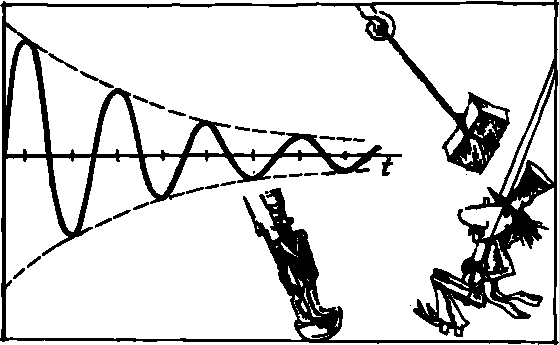
\includegraphics[width=\textwidth]{figures/fig-04-07.pdf}
\caption{A graph of a damped oscillation.}
\label{fig-4.07}
\end{figure}

Friction will significantly change any oscillations. In
the presence of friction, oscillations gradually damp. The
greater the friction, the faster the damping occurs. Try
making a pendulum immersed in water oscillate. It is
unlikely that you will succeed in getting the pendulum to
complete more than one or two oscillations. If a pendulum is immersed in a very viscous medium, there may fail to be any oscillation at all. The deflected pendulum will simply return to its equilibrium position. A typical graph for a damped oscillation is shown in \figr{fig-4.07}. The deviation from the equilibrium position has been plotted
along the vertical axis, and the time along the horizontal one. The amplitude of a damped oscillation diminishes with each oscillation.

\section{Resonance}

A child is seated on a swing. His feet do not reach the
ground. In order to swing him, one can, of course, raise
the swing high up and then let it go. But this would be
rather difficult and also quite unnecessary; it is enough
to gently push the swing in time with the oscillations,
and in a short time the child will be really swinging!

In order to swing a body, it is necessary to act in time
with the oscillations. In other words, it is necessary to
make one's pushes occur with the same period as that of
the free oscillations of a body. In such cases one speaks of
\emph{resonance}.

Resonance, widespread in nature and technology, merits careful consideration.

You can observe a very amusing and peculiar occurrence of resonance if you construct the following apparatus. Extend a string horizontally and hang three pendulums on it (\figr{fig-4.08}), two short ones of identical length and a longer one. Now deflect and release one of the short pendulums. In a few seconds you will see how the other
pendulum of the same length will gradually begin oscillating too. A few more seconds -- and the second short pendulum will swing, so that it will no longer be possible to tell which of the two pendulums first began moving.
\begin{figure}[!ht]
\centering
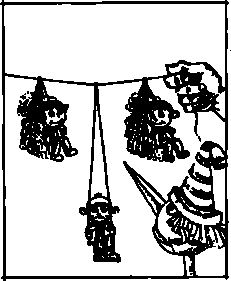
\includegraphics[width=0.6\textwidth]{figures/fig-04-08.pdf}
\caption{An apparatus for demonstrating resonance.}
\label{fig-4.08}
\end{figure}

What is the reason for this? Pendulums of the same
length have identical periods of free oscillations. The
first pendulum swings the second. The oscillations are transmitted from one to the other through the string connecting them. True, but there is yet another pendulum, of different length, hanging on the string. And what will happen to it? Nothing will happen to it. The period of this pendulum is different, and a short pendulum will not
be able to swing it. The third pendulum will be present
at this interesting energy ``transfusion'' from one pendulum to another, taking no part in it.

Each of us often comes across mechanical resonance
phenomena. Perhaps you simply did not pay any attention to them, even though resonance is sometimes very
bothersome. A streetcar passed by your window, and the
dishes in the sideboard began jingling. What is the matter? Oscillations of the ground were transmitted to the
building and simultaneously to the floor of your room,
so your sideboard and the dishes in it started to vibrate.
The oscillation was propagated so far and through so
many objects. This happened as a result of resonance.
The external oscillations were in resonance with the free
oscillations of the bodies. Almost any rattling which
we hear in a room, a factory or a car occurs because of
resonance.

Resonance, as, incidentally, many phenomena, can be
both useful and harmful.

A machine is standing on a mounting. Its moving parts
move rhythmically, with a definite period. Imagine that
this period coincides with that of free oscillation of the
mounting. What will happen? The mounting will be soon
vibrating, which could result in a breakdown.

The following fact is known. A company of soldiers
was marching in step across a bridge in St. Petersburg.
The bridge collapsed. An investigation into this matter
was begun. It seemed that there were no grounds for
anxiety over the fate of the bridge or the people: how
many times had crowds gathered on this bridge, had heavy
vehicles weighing much more than a company of soldiers
slowly crossed it!

But a bridge sags by an insignificant amount under the
action of a heavy weight. An incomparably greater sagging occurs when a bridge swings. The resonance amplitude of an oscillation can be thousands of times greater than
the displacement caused by a stationary load of the same
weight. This is precisely what the investigation showed --
the period of free oscillation of the bridge coincided with
that of an ordinary marching step.

Therefore, when a military subunit crosses a bridge,
a command is given to break step. If people's movements
are not coordinated, resonance will not set in and bridges
will not swing. Incidentally, this tragedy is well remembered by engineers. In designing bridges, they try to make its period of free oscillation far from the period of a marching step.

Designers of mountings have similar problems. They
try to make the mounting in such a way that its period
of oscillation be as far as possible from that of the moving
parts of a machine.
